%-----------------------------------LICENSE------------------------------------%
%   This file is part of Mathematics-and-Physics.                              %
%                                                                              %
%   Mathematics-and-Physics is free software: you can redistribute it and/or   %
%   modify it under the terms of the GNU General Public License as             %
%   published by the Free Software Foundation, either version 3 of the         %
%   License, or (at your option) any later version.                            %
%                                                                              %
%   Mathematics-and-Physics is distributed in the hope that it will be useful, %
%   but WITHOUT ANY WARRANTY; without even the implied warranty of             %
%   MERCHANTABILITY or FITNESS FOR A PARTICULAR PURPOSE.  See the              %
%   GNU General Public License for more details.                               %
%                                                                              %
%   You should have received a copy of the GNU General Public License along    %
%   with Mathematics-and-Physics.  If not, see <https://www.gnu.org/licenses/>.%
%------------------------------------------------------------------------------%
%       Author: Ryan Maguire                                                   %
%       Date:   2023/10/14                                                     %
%------------------------------------------------------------------------------%
\documentclass{article}
\usepackage[margin=1in]{geometry}
\usepackage{amssymb}
\usepackage{amsthm}
\usepackage{amsmath}
\usepackage{graphics}
\usepackage{hyperref}

\hypersetup{colorlinks=true, linkcolor=blue}

\theoremstyle{plain}
\newtheorem{theorem}{Theorem}
\newtheorem{conjecture}{Conjecture}
\newtheorem{question}{Question}

\title{Research Statement}
\author{Ryan Maguire}
\date{\today}

\begin{document}
    \maketitle
    \section{Introduction}
        My research interests lie in knot theory, topology, and Lorentz
        geometry, with a particular captivation in numerical methods and the
        design of algorithms. Knot theory is a challenging field when it comes
        to numerical analysis, many of the procedures have aweful complexities.
        For a simple example, it has been known since the 1920s
        (Reidemeister \cite{Reidemeister1927}, Alexander and Briggs
        \cite{AlexanderBriggs1926}) that two knot diagrams are isomorphic as
        knots if and only if there is a finite sequence of Reidemeister moves
        between them. In \cite{HassLagarias2001} Hass and Lagarias found an
        explicit upper bound for the number of moves required to convert an
        unknot with $n$ crossings to it's usual zero-crossing diagram. The
        bound is $2^{cn}$ where $c$ is the constant $10^{11}$.%
        \footnote{%
            The authors remarked that this can be improved.
            If we input $n=1$ we get an upper bound of
            $2.5\times{10}^{30,102,999,566}$ Reidemeister moves,
            when the minimum required is 1!
        }
        Heinrich and Kauffman found a factorial expression that only grows
        larger than this exponential formula for knots with more than
        $10^{10^{10}}$ crossings \cite{HenrichKauffman2010Unknotting}, and
        more recently a polynomial bounded of
        $(236n)^{11}$ was found by Lackenby \cite{Lackenby2015Unknotting}.
        \par\hfill\par
        A simple algorithm for detecting if any knot diagram corresponds to the
        unknot can be made using these bounds. Loop through all possible
        combinations of Reidemeister moves of length $(236n)^{11}$ for your
        initial $n$ crossing knot diagram, and if never
        find the standard diagram for the unknot you know you've got something
        different. In practice the universe will reset itself before you're
        algorithm terminates when implemented on real hardware.%
        \footnote{%
            There are around $3^{(236n)^{11}}$ combinations of Reidemeister
            moves. Inputting $n=2$ yields roughly $10^{10^{29}}$ combinations
            to check. The age of the universe is about $10^{18}$ seconds.
        }
        Other methods must be devised to make this problem approachable.
        In 2011 Kronheimer and Mrowka proved that Khovanov homology detects the
        unknot \cite{KronheimerMrowka2011KhovanovUnknot} and Bar-Natan's 2006
        paper provides an efficient means of computing this
        \cite{BarNatan2006FASTKH}, running (experimentally) like
        $O(2^{\sqrt{n}})$ where $n$ is the number of crossings. Most recently
        Lackenby developed an algorithm that runs in
        $O(2^{\log(n)^{3}})$, quasi-polynomial time
        \cite{LackenBy2021QuasiPolyUnknotting}. The complexity of this problem
        has been well studied. In 2014 Kuperberg proved (assuming the generalized
        Riemann hypothesis is true) that knottedness is both \texttt{NP} and
        \texttt{co-NP} \cite{Kuperberg2014KnottednessNP}. Lackenby soon after
        proved the same result without the assumption of the generalized
        Riemann hypothesis \cite{Lackenby2021UnknotNP}.
        \par\hfill\par
        The above paragraphs should convince one that even simple problems
        (recognizing the unknot) in knot theory are challening,
        both theoretically (performing the mathematics and designing the
        algorithms), and practically (implementing the algorithms
        in a programming language).
        My personal contributions lie in the implementation of knot algorithms
        for the tabulation of knot invariants. For a simple example,
        consider the Jones polynomial. Given an $n$ crossing knot $K$
        with crossings ordered between $0$ and $n-1$ we can defined the
        Kauffman bracket via:
        \begin{equation}
            \langle{K}\rangle(q)
            =\sum_{k=0}^{2^{n}-1}(-q)^{w(k)}(q+q^{-1})^{c(k)}
        \end{equation}
        Where $w(k)$ is the Hamming weight of $k$, the number of 1's that occur
        in the binary expansion of $k$, and $c(k)$ is the
        \textit{circle counting function}. That is, given a number
        $0\leq{k}\leq{2}^{n}-1$ we write $k$ in binary. If the $m^{th}$ bit is
        zero we performed a zero-smoothing at the $m^{th}$ crossing of $K$,
        otherwise we perform a one-smoothing. Every bit of $k$ tells us how to
        smooth all of the crossings (See Fig.~\ref{fig:cube_of_resolutions}).
        \begin{figure}
            \centering
            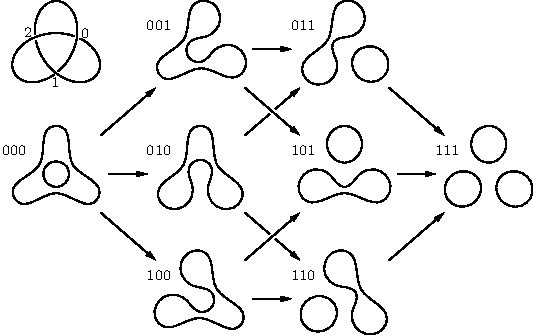
\includegraphics{trefoil_knot_cube_of_resolutions.pdf}
            \caption{Cube of Resolutions for the Trefoil}
            \label{fig:cube_of_resolutions}
        \end{figure}
        The result is the disjoint union of
        cycles in the plane. $c(k)$ counts the number of cycles corresponding
        to $k$. The Jones polynomial $J(K)$ is a normalization of
        $\langle{K}\rangle$ in terms of the writhe of $K$. The normalization
        step runs in constant time
        (shifting the minimum degree of the polynomial) and can be ignored for
        the purposes of algorithm design. The na\"{i}ve brute-force formula
        above yields an algorithm that is $O(2^{n})$, assuming that
        polynomial multiplication and addition run in constant time.
        Many improvements have been made over the years, and several
        algorithms exist (\cite{Thistlethwaite1987SpanningTreeJones},
        \cite{Zulli1995MatrixForJonesPolynomial},
        \cite{ElMisieryElHorbatyJonesAlgorithm},
        \cite{Gousbet2001JonesAlgorithm},
        \cite{MustafaLevitt2018JonesAlgorithm}), and even quantum algorithms
        exist (See \cite{JonesQuantumAlgorithm} and \cite{Lomonaco2008AQM}).
        Implementations have been made
        and optimized (\cite{sage}, \cite{regina},
        \cite{SnapPy}, \cite{libtmpl})
        allowing for the tabulation of the Jones polynomial of
        all prime knots with up to 19 crossings
        \cite{JonesData}. Similar efforts exist for the HOMFLY-PT polynomial
        (\cite{Gousbet1999HOMFLYAlgorithm},
        \cite{Burton2018HOMFLFixedParameter},
        \cite{Burton2012ComputationalTW}),
        a bivariate Laurent polynomial that generalizes the Jones polynomial,
        and a database has been created (\cite{HOMFLYData}). The Khovanov
        polynomial, defined from Khovanov homology by throwing away the torsion
        components, summing over the dimension of the homogeneous components
        $KH_{n}^{m}(K)$:
        \begin{equation}
            Kh(K)(q,\,t)=\sum_{m,\,n}
                q^{n}t^{m}\textrm{dim}\big(KH_{n}^{m}(K)\big)
        \end{equation}
        This contains the Jones polynomial, $J(K)(q)=Kh(q,\,-1)$. Efforts to
        tabulate the Khovanov polynomial have proven difficult, but all prime
        knots up to 17 crossings have been completed
        \cite{KhovanovData}.
        \par\hfill\par
        I have used these tables and programs to experiment with conjectures in
        knot theory and contact topology. A contact structure on a
        $2n+1$ dimensional manifold $M$ is a distribution of hyperplanes in the
        tangent bundle of $M$ satisfying a \textit{maximal non-integrability}
        condition. Locally this means it is given by a 1-form $\alpha$ such
        that $\alpha\land(\textrm{d}\,\alpha)^{n}\ne{0}$. The standard contact
        structure on $\mathbb{R}^{3}$ can be given globally by
        $\alpha=\textrm{d}z-y\textrm{d}x$, the hyperplane at $(x,\,y,\,z)$
        being spanned by the vectors $\partial_{x}+y\partial_{z}$ and
        $\partial_{y}$ (See Fig.~\ref{fig:darboux_form}). The maximal
        non-integrability conditions means that there is no surface that,
        neither locally nor infinitesimally, has its tangent planes given by
        the hyperplane distribution.
        \begin{figure}
            \centering
            \resizebox{0.8\textwidth}{!}{%
                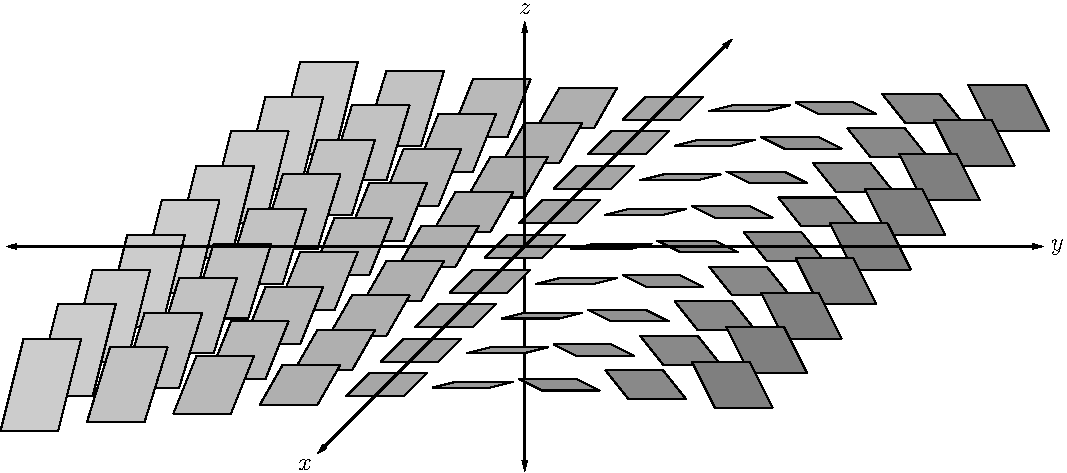
\includegraphics{darboux_form_001.pdf}
            }
            \caption{Standard Contact Structure for $\mathbb{R}^{3}$}
            \label{fig:darboux_form}
        \end{figure}
        It is, however, possible for curves to be everywhere tangent to the
        contact structure. These are called \textit{Legendrian submanifolds}.
        Legendrian knots are smooth embeddings of $\mathbb{S}^{1}$ into
        $\mathbb{R}^{3}$ that are also Legendrian submanifolds. Legendrian
        knot theory studies Legendrian knots up to \textit{Legendrian isotopy},
        a smooth family $H_{t}$, $t\in[0,\,1]$, of Legendrian knots. It is
        possible for two embeddings of $\mathbb{S}^{1}$ into $\mathbb{R}^{3}$
        to be equivalent topologically as knots, but not as Legendrian knots.
        \par\hfill\par
        Legendrian knot invariants exist, such as the Thurston-Bennequin $tb$
        number, and the rotation number $r$ (these are not invariants of
        topological knots). A topological knot type $K$ is said to be
        \textit{Legendrian simple} if all Legendrian representations of $K$ are
        uniquely determined by the ordered pair $(tb,\,r)$. Several families of
        knots are known to be Legendrian simple, such as the torus knots,
        and \textit{half} of the twist knots ($K_{m}$ for all $m\in\mathbb{Z}$
        with $m\geq{-3}$).
        \par\hfill\par
        In \cite{ChernovMaguireLegendrianConjecture} Chernov and I conjectured
        that Khovanov homology is able to detect Legendrian simple knots. This
        would generalize the works of Kronheimer and Mrowka
        \cite{KronheimerMrowka2011KhovanovUnknot},
        Baldwin and Sivek \cite{BaldwinSivekKhovanovTrefoils}, and
        Baldwin, Dowlin, Levine, Lidman, and Sazdanovi
        \cite{BaldwinDowlinKhovanovFigureEight}, who proved that Khovanov
        homology detects the unknot, trefoils, and figure-eight knot,
        respectively, the simplest of the Legendrian simple knots.
        \par\hfill\par
        Using the torus knots, twist knots, and even the conjectured Legendrian
        simple knots in \cite{LegendrianKnotAtlas}, we compared the Jones
        polynomial of all prime knots with up to 19 crossings against these.
        Several matches were found, and since the Khovanov polynomial contains
        the Jones polynomial (recall $J(K)(q)=Kh(q,\,-1)$), these matches are
        the only possible candidates for matching Khovanov homologies. Upon
        computing these, the following was found (by brute force).
        \begin{theorem}
            If a prime knot $K$ has less than or equal to 19 crossings and has
            the Khovanov homology of a torus knot or a twist knot $T$,
            then $K$ is equivalent to $T$.
        \end{theorem}
    \section{Previous Work}
        \subsection{DWEL}
            The first \textit{real} project I worked on was DWEL, the
            Dual Wavelength Echidna LIDAR
            (\textbf{LI}ght \textbf{D}etectction \textbf{A}nd \textbf{R}anging),
            described in \cite{DWEL2012}.
            By using two lasers at 1064 nm and 1548 nm the instrument is able
            to distinguish scattering from leaves and tree trunks. This allows
            the mapping of forests for botanical studies. I, Glenn Howe, and
            Kuravi Hewawasum worked on this at the Center for Atmospheric
            Research (CAR) in Lowell, MA, in collaboration with UMass Boston
            and Boston University, and the device saw uses in California,
            Harvard forest, and Australia
            \cite{Li2016RadiometricCO}.
        \subsection{HiT\&MIS}
            The bulk of my work at CAR, renamed LoCSST
            (Lowell Center for Space Science and Technology), was on
            HiT\&MIS, a spectrometer used to study the aurora borealis
            (\cite{HiTandMIS2011}, \cite{2011AGUFMSA13B1890C},
            \cite{2014AGUFMSA13B4000H}, \cite{2015AGUFMSA13B2369A}). The
            instrument used an echelle grating to achieve a high dispersion
            order allowing several wavelengths of light to be detected and
            differentiated between. Two copies of the instrument were built
            and deployed in parallel with Dartmouth's BARREL mission in
            Kiruna, Sweden.
        \subsection{SPINR}
            The final project I worked on was the analysis of data from the
            SPINR sounding rocket mission.
        \subsection{Cassini}
            After leaving Lowell I accepted a position at Wellesley college
            working with the team leader for the radio science portion of NASA's
            Cassini mission. Here I studied and implemented algorithms in
            Fourier analysis, Fredholm equations, and general inverse problems.
            These efforts were a part of \texttt{rss\_ringoccs}, an open source
            package for analyzing the occultation data for the rings of Saturn
            \cite{rssringoccs}. Fourier optics tell us that the diffraction
            pattern of a radio signal passing through an aperture can be
            modeled via:
            \begin{equation}
                \hat{T}(\rho_{0},\,\phi_{0})=
                    \frac{\sin(B)}{i\lambda}
                    \int_{0}^{\infty}
                    \int_{0}^{2\pi}
                        \frac{\rho}{D}
                        T(\rho,\,\phi)
                        \exp\big(i\psi(\rho,\,\phi,\,\rho_{0},\,\phi_{0})\big)\;
                    \textrm{d}\,\rho\;
                    \textrm{d}\,\phi
            \end{equation}
            where $\lambda$ is the wavelength of the incident light, $B$ is
            the angle the ray makes with the aperture, $(\rho_{0},\,\phi_{0})$
            is the point of interest, $(\rho,\,\phi)$ is the dummy point of
            integration, $T$ is the transmittance of the aperture, $\psi$ is
            the Fresnel kernel, and $D$ is the distance from the observer to
            the point $(\rho_{0},\,\phi_{0})$. Assuming a cylinderically
            symmetric aperture (like the rings of Saturn),
            the transmittance function $T$ may be written
            $T(\rho_{0},\,\phi_{0})=T(\rho_{0}$. Since the integrand involves a
            term of the form
            $\exp\big(i\psi(\rho,\,\phi,\,\rho_{0},\,\phi_{0})\big)$ we may
            invoke the stationary phase approximation to rid ourselves of the
            integral over the angle. The reduction leads us to:
            \begin{equation}
                \hat{T}(\rho_{0})=
                    \int_{0}^{\infty}
                        \frac{1-i}{2F}
                        T(\rho)
                        \exp\big(i\psi(\rho,\,\phi,\,\rho_{0},\,\phi_{0})\big)\;
                    \textrm{d}\,\rho
            \end{equation}
            where $F$ is the \textit{Fresnel scale}, given by the formula:
            \begin{equation}
                F=\Big(
                    \frac{\lambda{D}}{2}
                    \frac{1-\cos^{2}(B)\sin^{2}(\phi_{0})}{\sin^{2}(B)}
                \Big)^{1/2}
            \end{equation}
            The classic Fresnel approximation treats $F$ as constant and
            approximates $\psi$ with a quadratic. The resulting equation
            \begin{equation}
                \hat{T}(\rho_{0})=
                    \frac{1-i}{2F}
                    \int_{0}^{\infty}
                        T(\rho)
                        \exp\Big(\frac{i\pi}{2}
                            \big(\frac{\rho-\rho_{0}}{F}\big)^{2}
                        \Big)\;
                    \textrm{d}\,\rho
            \end{equation}
            is invertible, by the convolution theorem,
            and the inverse is given by:
            \begin{equation}
                T(\rho)=
                    \frac{1+i}{2F}
                    \int_{0}^{\infty}
                        \hat{T}(\rho_{0})
                        \exp\Big(
                            -\frac{i\pi}{2}\big(\frac{\rho-\rho_{0}}{F}\big)^{2}
                        \Big)\;
                    \textrm{d}\,\rho_{0}
            \end{equation}
            This formula mimics the inverse Fourier transform. It suggests a
            numerical approximation for the general formula:
            \begin{equation}
                T(\rho)\approx
                    \frac{1+i}{2F}
                    \int_{0}^{\infty}
                        \hat{T}(\rho_{0})
                        \exp\big(
                            -i\psi(\rho,\,\phi,\,\rho_{0},\,\phi_{0})
                        \big)\;
                    \textrm{d}\,\rho_{0}
            \end{equation}
            \texttt{rss\_ringoccs} implements the above work and has been
            highly optimized over the past few years to very efficiently
            process the data. All of the occultation observations from Cassini
            can be processed in about 20 minutes on a decent computer
            (my initial code from 2017 took 130+ hours on that same computer).
            This has been used to study the rings and led to
            \cite{FRENCH2023115678} and \cite{NICHOLSON2023115287}.
    \section{Future Work}
    \newpage
    \bibliographystyle{plain}
    \bibliography{bib.bib}
\end{document}
